\documentclass[11pt,a4paper,english]{article}
\usepackage[utf8]{inputenc}
\usepackage[T1]{fontenc}
\usepackage{amsfonts,amsmath,amssymb,pifont,enumerate,graphicx,textcomp,varioref,algpseudocode,listings}
\usepackage[margin=1in,footskip=0.25in]{geometry}

\title{MEK3220 - Formulae sheet}
\author{Krister Stræte Karlsen}
\tolerance = 5000 
\hbadness = \tolerance 
\pretolerance = 2000 

\usepackage{wrapfig}
\usepackage{color}
\usepackage{listings}
\usepackage{setspace}
\usepackage{framed}

\begin{document}
\maketitle

{\scshape The displacement gradient} 
\begin{align*}
\nabla \mathbf{u} = 
\begin{pmatrix}	    \frac{\partial u_x}{ \partial x} & \frac{\partial u_x}{ \partial y} & \frac{\partial u_x}{ \partial z}      \\
                		\frac{\partial u_y}{ \partial x} & \frac{\partial u_y}{ \partial y} & \frac{\partial u_y}{ \partial z}     \\
               	 	\frac{\partial u_z}{ \partial x} & \frac{\partial u_z}{ \partial y} &\frac{\partial u_z}{ \partial z}     
\end{pmatrix}
\end{align*}
\hspace{1cm} For $ \nabla \mathbf{u} =  ( \nabla \mathbf{u})^T  $ we have that $\nabla \mathbf{u} = \epsilon $, the \emph{strain tensor}.\\

{\scshape Strain tensor} 
\begin{align*}
\epsilon = \frac{1}{2}(\nabla \mathbf{u} + \nabla \mathbf{u}^T  ) 
\end{align*}

{\scshape Hooke's law} 
\begin{align*}
\sigma  = \lambda tr(\epsilon) I + 2\mu \epsilon 
\end{align*}

{\scshape Inverted Hooke's law} 
\begin{align*}
\epsilon = \frac{1+\nu}{E}\sigma - \frac{\nu}{E} tr(\sigma)I   
\end{align*}

{\scshape Cauchy's equilibrium equation} 
\begin{align*}
\mathbf{f_v} + \nabla \cdot \sigma = 0
\end{align*}

{\scshape Equation of continuity} 
\begin{align*}
\frac{\partial \rho}{\partial t} + \nabla \cdot  \rho \mathbf{v} = 0
\end{align*}

{\scshape Isotropic viscous stress} 
\begin{align*}
\sigma = pressure + \textit{shear stress} =  (-p)I + \mu (\nabla \mathbf{v}  + \nabla \mathbf{v}^T  )
\end{align*}

{\scshape Navier-Stokes} 
\begin{align*}
\frac{d \mathbf{v}}{dt} + (\mathbf{v} \cdot \nabla)\mathbf{v} = \mathbf{g} - \frac{1}{\rho} \nabla p + \nu \nabla^2 \mathbf{v}, \quad \nabla \cdot \mathbf{v} = 0  
\end{align*}

{\scshape Navier's equation for elastic media in motion} \\
\begin{align*}
\rho \frac{\partial^2 \mathbf{u}}{\partial t^2} = \mu \nabla^2 \mathbf{u} + (\lambda + \mu) \nabla ( \nabla \cdot \mathbf{u}) + \mathbf{f_v}
\end{align*}

{\scshape Lamè coefficients} 
\begin{align*}
E=\mu \frac{3\lambda + 2\mu}{\lambda + \mu}, \quad \nu = \frac{\lambda}{2(\lambda + \mu)}
\end{align*}
\begin{align*}
\lambda = \frac{E \nu}{(1-2\nu)(1+\nu)}, \quad \mu = \frac{E}{2(1+\nu)}
\end{align*}

\vspace{1cm}

{\scshape Energy equations} \\

\underline{Kinetic energy}(per volume) for fluid:
\begin{align*}
E_k = \frac{1}{2} \rho \mathbf{v}^2 = \frac{1}{2} \rho (u^2 + v^2 + w^2) 
\end{align*}

\underline{Work} done by wall(at $y=h$ with length: $L$) from shear stress($\sigma_{xy}$) on fluid:
\begin{align*}
W = U(h) L \sigma_{xy}(h)
\end{align*}

\underline{Dissipation}
\begin{align*}
\Delta = 2 \mu [\frac{1}{2} (\nabla \mathbf{v}  + \nabla \mathbf{v}^T  ) ]^2
\end{align*}

\underline{Heat transfer equation}
\begin{align*}
\rho c \left(\frac{\partial T}{\partial t} + (\mathbf{v} \cdot \nabla)T \right) = k \nabla^2 T + h + \Delta 
\end{align*}

\vspace{1cm}

{\scshape Stress relations} \\

\begin{wrapfigure}{R}{0.5\textwidth}
\centering
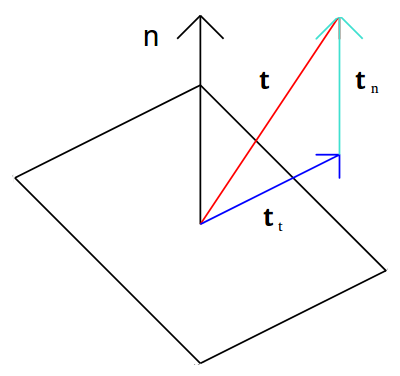
\includegraphics[width=0.35\textwidth]{figures/stressplane.png}
\end{wrapfigure}

\underline{Stress on surface} (red)
\begin{align*}
\mathbf{t} =\sigma \cdot \mathbf{n}
\end{align*}

\underline{Normal stress on surface} (light blue)
\begin{align*}
\sigma_{n} =\mathbf{t} \cdot \mathbf{n} \\ 
\mathbf{t}_n = \sigma_{n} \mathbf{n}
\end{align*}

\underline{Shear stress on surface} (blue)
\begin{align*}
\mathbf{t}_t = \mathbf{t} - \mathbf{t}_n 
\end{align*}


%{\scshape Beam equations} \\
%
%\emph{Euler-Bernoulli} and some additional important relations
%
%\begin{figure}[h!]
%\centering
%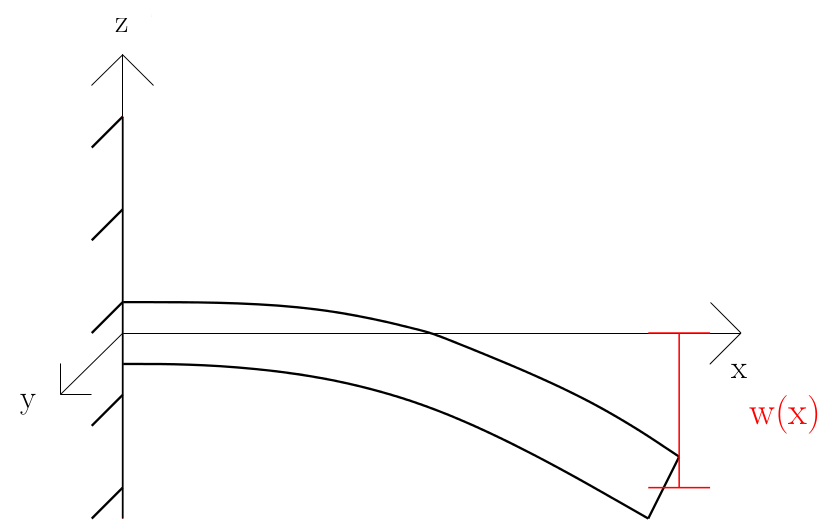
\includegraphics[scale=0.15]{figures/beam.png}
%\end{figure}
%
%\begin{align*}
%\frac{d^2 w(x)}{dx^2} = - \frac{M_y (x)}{EI}, \quad \frac{dM_y(x)}{dx} = F_z, \quad \frac{dF_z}{dx} = - F_{ext}^{(z)} 
%\end{align*}


\end{document}



\grid
